% https://github.com/MCG-NKU/NSFC-LaTex
% by Ming-Ming Cheng https://mmcheng.net
% 关于VsCode LaTeX的配置 https://www.cnblogs.com/ourweiguan/p/11785660.html
% Windows下Tex Live最新版可以用pdfLatex快速编译和标准模板相似度更高的文档。



\documentclass[12pt]{article}


\usepackage{nsfc}
\usepackage{booktabs}
\usepackage{multirow}
\usepackage{graphicx}
\usepackage{subcaption}
\usepackage{amsmath}
\setmainfont{Times New Roman}

%\usepackage{fontspec}
%\usepackage{xcolor}
%\defaultfontfeatures{Ligatures=TeX}

\newcommand{\addImg}[2][1.0]{\includegraphics[width=#1\linewidth]{#2}}
\newcommand{\cmm}[1]{\textcolor[rgb]{0,0.6,0}{CMM: #1}}
\newcommand{\todo}[1]{{\textcolor{red}{\bf [#1]}}}
\newcommand{\myPara}[1]{\paragraph{#1：}}
\newcommand{\myEmph}[1]{\textbf{\textcolor[rgb]{0,0,0.25}{#1}}}
\newcommand{\mySec}[1]{\vspace{0.15in} \noindent \myEmph{$\square$~#1}}

\DeclareMathOperator*{\argmax}{arg\,max}  % define once in preamble

\graphicspath{{figures/}}


\begin{document}




%\if 0
\begin{center}\bf\Large 开放环境下3D点云测试时自适应分析方法研究 \\

Research on Test-time Adaptation for 3D Point Cloud Analysis in Open World 
\end{center}





\textbf{摘要}：
%
“用……方法（手段）进行……研究，探索/证明……问题，
对阐明……机制／揭示……规律有重要意义，为……奠定基础／提供……思路 ”。
作用：画龙点睛。
效果：引发评议专家兴趣，使其产生探个究竟的好奇心——“他到底要怎么做？”
摘要字少，但切忌平淡无奇（要勾起评委浓厚兴趣）。
\myEmph{一定要语气坚定，旗帜鲜明，字数有限，资源宝贵，要特别注意重点突出，
讲明现状、意义、课题主要研究目标、内容、思路和预期结果}。



\textbf{Abstract}：
***


科学问题属性：聚焦前沿，独辟蹊径



【待补充】


\clearpage
%\fi


%%%%%%%%% TITLE
\title{报告正文}

\maketitle
\thispagestyle{empty}

%\emph{\large 参照以下提纲撰写，要求内容翔实、清晰，层次分明，标题突出。
%\nsfClr{请勿删除或改动下述提纲标题及括号中的文字。}}


\ContentDes{（一）立项依据与研究内容\textnormal{\alert{（建议$8000$字以内）}}：}


\NsfcSection{1}{项目的立项依据}{
（研究意义、国内外研究现状及发展动态分析，需结合科学研究发展趋势来论述科学意义；
或结合国民经济和社会发展中迫切需要解决的关键科技问题来论述其应用前景。
附主要参考文献目录）；}

% 写作思路是什么
% 1. 倒推 
% 1.1 本研究到底要解决什么问题？    ->  开放环境下点云处理方法效果差的问题，这里最好用数据说明
% 1.2 我提出了什么方案？           ->  测试时自适应缓存模型
% 1.3 提出的方案有何好处？         ->  拔插即用/免训练/高效/在线性能提升

% 2. 正推
% 2.1 简述研究背景
% 2.2 该背景下重点关注什么任务？
% 2.3 已有方法是怎么做的？存在什么问题？
% 2.4 本项目的解决思路      ->      主要讲思想
% 2.5 本项目的技术方案      ->      主要讲技术路径
% 2.6 提出的解决方案有何优势？
% 2.7 提出的解决方案有何科学意义和重要价值


\subsection{研究背景及科学意义}

% 3D点云+ 3D感知任务的重要性 
在数智化浪潮席卷全球的今天，如何精准地表征与感知真实物理世界，是机器视觉与人工智能领域面临的重要挑战。3D点云（******要画个图讲一下******）作为物理世界最直接、最精确的数字表征形态，相较于二维图像，蕴含着不可替代的几何结构与深度信息，能够有效克服光照变化、尺度歧义等局限。因此，基于3D点云的高精度感知任务
——涵盖三维物体识别、检测与场景语义分割——构成了机器理解复杂物理现实的核心能力，是连接数字虚拟空间与实体物理世界的关键纽带。（******再画个图讲一下点云感知任务******）

% 讲强大感知能力的重要性
这种对三维空间精确、实时的感知与理解能力，绝不仅仅是单纯的数据处理，而是实现更高阶“空间智能（Spatial Intelligence）”的基石与第一步。只有当智能体具备了类似于人类的“空间之眼”，能够准确把握物理对象的属性及其在空间中的位置关系，才能进一步在此基础上进行复杂的空间推理、路径规划与实体交互，从而真正实现从被动地“看清世界”到主动地“融入世界”的跨越。

% 讲空间智能的重要性
“空间智能”这一前沿概念由世界知名人工智能专家、斯坦福大学教授李飞飞率先提出，被视为系语言智能之后，人工智能发展的下一个重要里程碑~\cite{li25spatialai}。李飞飞教授强调了AI系统不仅要处理符号和二维图像，更要在真实的三维物理世界中具备感知、理解、推理与交互的核心能力。当前，国内外术界与产业界已形成广泛共鸣：人工智能必须走出屏幕，走向物理实体，发展能够适应复杂物理环境的智能。

% 国家政策层面的意义
空间智能的研究对于推动自动驾驶、智能制造、人形机器人等前沿领域的突破具有决定性意义。同时，空间智能的发展与国家政策导向高度契合，2025年8月国务院印发的《关于深入实施“人工智能+”行动的意见》明确提出要将人工智能与各行各业深度融合，促进生产力革命性跃迁，赋能实体经济。

% 如何过渡到本项目的挑战？
%   引出当前面临的挑战性问题
%   挑战说得比较简单，一句话就带过了，需要展开
%   展开的时候需要明确，与下文研究内容一一对应
然而，将3D点云感知系统真正部署于开放、动态的现实物理环境（Open Environment）中，面临着巨大的挑战。

\myEmph{挑战1:} 现有方法多数在封闭数据集上训练点云感知模型，局限于训练数据见过的物体和类别，未能赋予模型对未知环境中新物体、新类别、新场景语义理解能力，不能很好扩展到开放环境。

\myEmph{挑战2:} 现有方法未充分考虑测试数据分布特性，大多做法是为每个测试样本单独生成预测结果，导致点云感知模型在推理和部署阶段缺乏对测试数据和未知环境的理解，显著影响模型的自适应能力。

\myEmph{挑战3:} 现有方法未能设计系统性的测试时自适应策略，在未知环境包含大量噪声，发生数据分布漂移和坍塌时缺乏有效应对策略，难以满足实际应用对准确性、鲁棒性、高效性的要求。

% 现有模型大多基于封闭数据集训练，一旦遇到未知的场景、天气或传感器噪声，往往因数据分布差异而导致性能显著下降，难以满足实际工业与社会应用对准确性、鲁棒性与安全性的严苛要求。

% 本项目研究思路
%   分别对应上述3个挑战
在此背景下，本项目应运而生，目标是将封闭设定的点云感知方法扩展到真实的开放环境，并设计一种通用的自适应策略大幅加强点云感知方法在测试和部署阶段的自适应能力，为空间智能的研究和发展提供基础支撑。
本项目拟采用循序渐进的方式研究开放环境下3D点云感知方法的自适应问题：
（1）首先探讨具有语义表达能力的点云编码问题，赋予3D点云感知模型识别未知环境中新物体、新类别、新场景的能力；
（2）在此基础上，研究在线捕获点云测试数据分布特性的方法，动态分析并掌握测试数据特点是模型在未知环境进行自适应调整的重要依据；
（3）在此基础上，探讨训练好的点云感知模型在推理和部署阶段的测试时自适应策略，以实现更好的测试时准确性、鲁棒性、泛化性。



\subsection{国内外研究现状}
% 从这几方面展开，提供参考文献
% 讲开放环境点云处理
%   讲明白过去的范式是怎么样的？特定数据集上训练模型，特定数据集上测试
%   讲明白现在朝着开放世界模型走？
%   存在的问题：鲁棒性/泛化性差/效率低
2017年，以PointNet~\cite{qi17pointnet,qi17pointnet2}为代表的深度点云处理方法横空出世，它们在点云物体识别、语义分割等
任务上的性能大幅超越人工特征工程和传统机器学习方法，（用ModelNet举例子，比传统方法好多少）。经过多年的发展，深度点云处理方法在
特定数据集（封闭设定）的性能趋于饱和（给出具体例子+图表，发表了多少篇论文，性能增益不到 6\%），
从2022年开始，越来越多的工作关注开放环境下点云处理问题，比如开放词表的点云识别~\cite{zhang22pointclip,zhu23pointclip2,xue23ulip,xue24ulip2,liu23openshape,zhou24uni3d}、
物体检测~\cite{zeng23clip2,zhu23pointclip2,lu23ov3det,cao23coda,yang24imov3d,cao25codav2}、语义分割，
当前该领域的研究重点已经从封闭数据集的设定迈向开放环境，且逐渐成为国内外一个前沿研究问题。

% 进一步讲开放环境的点云理解现状，存在什么问题
%   存在的挑战一句话就说完了，得扩充和丰富
但当前点云处理方法未能良好应对开放环境下的种种挑战，模型的准确性和鲁棒性非常脆弱（这里要举例子，至少目前看到这么多点云识别/检测的例子，准确性只有那么点），
不能满足实际应用需求。例如，当前最好的开放词表的点云物体检测模型 CoDA v2~\cite{cao25codav2}，在公开的ScanNet数据集上的平均精度 mean Average Precision (mAP@IoU$_{25}$) 仅为 22.72\%，
而在封闭数据集上训练的3DETR~\cite{misra213detr}模型在ScanNet的 mAP@IoU$_{25}$ 达到62.7\%，当前经过封闭数据训练的最佳方法Dest~\cite{wang25dest}在ScanNet达到了 78.3\% mAP@IoU$_{25}$ 的检测精度，领先CoDA v2 55.58\%个绝对点。

% 讲本项目思路
%   解释本项目涉及到的关键技术，就是下面列的
针对这些问题，本项目提出开放环境下基于缓存模型的测试时自适应点云分析方法，致力于提升开放环境下点云分析方法的鲁棒性和泛化能力。

\myEmph{上一段和下一段逻辑连贯性不好，尤其是下一段开头，在上面已经讲过了}

% 讲测试时自适应
%   讲主要思想，这要结合文献
尽管模型在训练阶段要尽可能学习各种情况，但现实世界是千变万化的，总有些新的数据特性在测试和部署阶段出现，
此时训练好的模型不再具备大规模重训练可行性，对于测试环境的应变能力和自适应能力显得尤为重要。
而测试时自适应技术旨在让模型在线运行时具备适应测试环境或根据测试数据特点调整自身预测的能力~\cite{yeo23rna}。
%   讲技术分类，也要总结文献
测试时自适应技术可大致分为两类，一类是需要根据测试样本调整预训练模型参数的~\cite{schneider20improving,wang21tent,zhang21adaptive,zhang22memo,shu22tpt,feng23difftpt,niu23towards,chen22adacontrastive,zhao2024rlcf}，另外一类是免训练的~\cite{wang24bftt3d,karmanov24tda,zanella24meanshift,farina24zero,sun25pointcache,tamjidi2025uniadapter}。在第一大类方法中，有调整BN层统计信息的~\cite{schneider20improving,wang21tent,zhang22memo}，有调整提示词的~\cite{shu22tpt,feng23difftpt}，还有调整模型其他部分参数（如图像编码器）的~\cite{zhang21adaptive,chen22adacontrastive,zhao2024rlcf}；在第二大类方法中，大部分是基于缓存模型的~\cite{wang24bftt3d,karmanov24tda,sun25pointcache,tamjidi2025uniadapter}，还有些经过理论推导进行数值变换的~\cite{zanella24meanshift,farina24zero}。

% 讲缓存模型——测试时自适应方法的一种
%   讲主要思想，就这一句话吗？不止这样吧，没把精华讲出来
缓存模型通过存储典型样本数据为模型在评测和部署时作参考。
%   讲技术路线分类？
这种思路和技术手段已在多种任务重得到体现和应用，比如语言建模~\cite{vinyals16mn,grave17unbounded,merity17pointer,khandelwal20generalization}、图像识别~\cite{vinyals16mn,snell17prototypical,finn17maml,chen18a,chen21meta-baseline,choi22improving,iwasawa21t3a,zhang22tip-adapter,zhang23cafo,karmanov24tda}、点云处理~\cite{zhang23pointnn,tang24pointpeft,sun25pointcache,wang24bftt3d,tamjidi2025uniadapter}。
%   讲本文如何看待缓存模型  ->  检索增强范式

% 讲存在的问题？
%   评述总结，该把这部分写出来了，不能磨了
%   1. TTA 存在很多假设，限制了实际应用
%   2. TTA 效率低，不能实时运行
%   3. 缓存模型依赖训练数据构建
然而，当前的测试时自适应点云分析方法面临以下几方面挑战：
%   分别对应后面的主要研究内容
%   最后一定要有对挑战的总结描述
\begin{itemize}
    \item 当前测试时自适应点云分析方法大多限定在封闭数据集设置，仅能处理训练过程已经见过的物体和场景类型，不具备应对开放环境的自适应能力。
    \item 当前测试时自适应点云分析方法依赖大规模训练数据构建缓存，但是模型测试和部署阶段获取大量训练数据不太实际，而且测试数据展示的特性和训练数据可能很不相同，导致这类方法的鲁棒性和泛化能力较弱，且运行效率不高，难以投入实际应用。
    \item 当前开放环境下测试时自适应点云分析方法的研究处于早期阶段，基础理论尚不完备，关键方法和技术路线尚不成熟。
\end{itemize}

综上所述，开放环境下测试时点云处理的研究处于起步阶段，相关基础理论有待发展，对应技术路径亟待验证。本项目计划从理论和实践两个维度展开研究：

（1）从理论角度出发，开放环境下测试时自适应点云分析方法理论框架尚不清晰。

（2）从应用角度出发，缓存模型构建和更新不够准确和高效。

（3）从应用角度出发，开放环境下基于缓存模型的测试时自适应点云分析方法未形成体系。

\subsection{本人具备的研究基础}

本人博士期间围绕3D点云处理的准确性、运行效率、鲁棒性和泛化性进行深入研究，广泛阅读了领域文献，熟悉并掌握了主要技术路径和方法，提出了系列创新方案，以第一作者身份围绕该主题发表了5篇顶级国际会议和期刊论文~\cite{sun25pointcache,sun24point-prc,sun25vsformer,sun24ppt3d,sun23vipformer}，初步具备了执行本项目的研究基础和实践经验。
其中，发表在CVPR 2025的论文(Point-Cache)探讨了开放环境下点云识别模型测试时鲁棒性和泛化性问题；发表在 NeurIPS 2025 的论文(Point-PRC)探讨了3D大模型的领域泛化能力；发表在 ICRA 2024 的论文(PPT) 探讨了如何用参数和数据高效的方式激活多模态3D大模型的预训练知识，从而增强点云处理的效果和效率；发表在 ICRA 2023 的论文探讨了如何结合图像和点云两个模态的信息增强点云处理的性能和效率。

% 研究基础总结
本人将充分利用这些工作积累，深入研究开放环境下3D点云模型测试时自适应问题，努力突破其中的关键科学问题和技术挑战，给出适合3D点云大模型自适应部署的理论和实践方案，为Spatial AI的发展贡献力量。本项目预期产出的研究成果对于3D场景重建、3D物体生成、3D物体配准、VR/AR等领域也具有重要参考价值。

\subsection{国内外相关工作}

\textbf{开放环境下3D点云处理}
% 从哪讲起呢？把事情发展的原委讲出来，配上自身评述

近几年，以CLIP~\cite{radford21clip}和ALIGN为~\cite{jia21scaling}代表的视觉-语言对比预训练方法受到了广泛关注，在这种思路指导下训练的模型能进行开放集合的图像理解（如图像识别/语义分割/物体检测），并且表现出显著改善的泛化能力，极大扩展了之前仅在图像单一模态训练的模型的能力边界（后者仅能处理训练阶段见过的物体/语义类别）。受到这类工作的启发，开放环境下3D点云处理的研究逐渐兴起，当前呈现出蓬勃发展的趋势。

% 怎么和上述概览的逻辑接起来
%   介绍典型任务分类
开放环境下3D点云处理典型的任务包括3D点云识别~\cite{zhang22pointclip,zhu23pointclip2,sun25pointcache,sun24point-prc,sun24ppt3d,xue23ulip,xue24ulip2,liu23openshape,zhou24uni3d}、
% PointCLIP~\cite{zhang22pointclip},Point-Cache~\cite{sun25pointcache}, Point-PRC~\cite{sun24point-prc}, PPT~\cite{sun24ppt3d}, ULIP~\cite{xue23ulip}, ULIP-2~\cite{xue24ulip2}, OpenShape~\cite{liu23openshape}, Uni3D~\cite{zhou24uni3d}
3D点云物体检测~\cite{zeng23clip2,zhu23pointclip2,lu23ov3det,yang24imov3d,cao23coda,cao25codav2}、
% CLIP2~\cite{zeng23clip2} (Clip2: Contrastive language-image point pretraining from real-world point cloud data), PointCLIP V2~\cite{zhu23pointclip2}, OV-3DET~\cite{lu23ov3det}, ImOV3D~\cite{yang24imov3d}, CoDA~\cite{cao23coda}, CoDA v2~\cite{cao25codav2}
3D点云语义分割~\cite{jiang24ov3d,kolodiazhnyi2024oneformer3d,zhou2025pointsam,rusnak25haec,boudjoghra2025openyolo3d}等。
% OV3D: Open-Vocabulary 3D Semantic Segmentation with Foundation Models~\cite{jiang24ov3d}
% OneFormer3D~\cite{kolodiazhnyi2024oneformer3d}, 
% Point-SAM~\cite{zhou2025pointsam}, 
% HAECcity~\cite{rusnak25haec}
% Open YOLO 3D~\cite{boudjoghra2025openyolo3d}, 
%   总结每类任务特点 有什么特点呢？这就要自己琢磨了
这几类任务起来有很大差异，从数据规模和复杂度层面，3D点云识别涉及到物体级的点云数据，规模和复杂度相对较小，而3D物体检测和语义分割要处理场景级的点云数据，规模和复杂度较大，因此不同任务的处理方法也有较大差异。

%   评述这些工作与本项目的联系和区别
然而，上述开放集合的点云处理方法缺乏自适应能力，无法根据测试环境特点作出自适应调整，极大限制了3D点云处理方法在开放环境和真实世界的部署应用。本项目正是针对这种缺陷，研究开放环境下3D点云处理的自适应方法，让3D模型能够高效的根据测试数据特点调整自身预测，从而改善模型的准确性和鲁棒性。

\textbf{测试时自适应方法}
% 根据Point-Cache这篇文章的思路，分类总结
%   分成哪几类呢？
%   - 2D TTA：
%       1. 非开放环境   <-  基于单模态   
%       2. 开放环境     <-  多模态
%       - 用不用按照实现方案把技术分个类？上面的2类太简单？
%   - 3D TTA
%       1. 基于小模型：鲁棒性和泛化能力本身不强+不是开放环境
%       2. 依赖庞大训练集构建pipeline
%       3. 未利用测试数据分布

测试时自适应技术在图像处理领域已经得到体现和应用。早期的图像处理测试时自适应技术应用在图像单一模态~\cite{liang20shot,liang22source,wang21tent,zhang22memo,sun20ttt,liu21ttt++,gandelsman22ttt-mae,iwasawa21t3a,zhang22memo}，由于未引入灵活的语言模态，这类方法只能在封闭数据集上进行图像识别，不具备在真实开放世界中进行图像处理的能力。近年来，测试时自适应技术与主流视觉-语言模型结合，掀起了开放环境下多模态大模型测试时自适应方法研究的浪潮~\cite{shu22tpt,feng23difftpt,tsai24gda,karmanov24tda,zanella24meanshift,farina24zero,guan2025sca,cha2025snap}，这些工作大大突破了封闭数据集合的设定，使得视觉-语言多模态模型更加贴近实际应用。

% ====== 2D TTA: uni-modal, close set ======
    % Memo~\cite{zhang22memo}

    % Test-time classifier adjustment module for model-agnostic domain generalization~\cite{iwasawa21t3a} (neurips 2021)

    % Tent: Fully test-time adaptation by entropy minimization~\cite{wang21tent} (iclr 2020),

    % Do we really need to access the source data? Source hypothesis transfer for unsupervised domain adaptation.~\cite{liang20shot} (icml 2020),

    % Source data-absent unsupervised domain adaptation through hypothesis transfer and labeling transfer.~\cite{liang22source} (TPAMI 2022),

    % TTT: Test-time training with self-supervision for generalization under distribution shifts.~\cite{sun20ttt}

    % TTT++~\cite{liu21ttt++} (neurips 2021),
    % The norm must go on: Dynamic unsupervised domain adaptation by normalization.~\cite{mirza22dua} (CVPR 2022),

    % TTT-MAE~\cite{gandelsman22ttt-mae} (Test-Time Training with Masked Autoencoders, neurips 2022) 

% ====== 2D TTA: multi-modal, open set ======
    % TPT, DiffTPT, TDA, 
    % GDA: Generalized diffusion for robust test-time adaptation.~\cite{tsai24gda} (CVPR 2024), 

    % On the test-time zeroshot generalization of vision-language models: Do we really need prompt learning?~\cite{zanella24meanshift} (CVPR 2024)

    % Zero~\cite{farina24zero}, SCA~\cite{guan2025sca}, SNAP~\cite{cha2025snap}

与在图像处理领域的探索相比，3D点云测试时自适应技术起步较晚，相关研究仍属于早期阶段。当前的技术流派可大致划分为三大类：第一类是基于小模型的方法~\cite{mirza23mate,wang24bftt3d,shim24cloudfixer}，这类方法首先仅局限于点云模态，缺乏开放集合的3D点云处理能力，其次由于模型本身能力有限，虽有测试时自适应技术加持，但展现的准确性和泛化能力不够；第二类是基于多模态大模型的方法~\cite{sun25pointcache,tamjidi2025uniadapter}，这类方法虽然能进行开放集合的点云处理，但是没有充分利用测试数据的分布特性（前/后面这段话是 **placehoder**），导致模型在现实世界测试和部署时鲁棒性和泛化能力仍不理想。

% ====== 3D TTA ======
% MATE, BFTT3D, CloudFixer, Point-Cache, Uni-Adapter

% 相关工作总结，本项目的特色之处

\textbf{缓存模型(与检索增强方法类比，并不等同)}
% 这部分放到测试时自适应中讲？还是单拎出来？
%   目前标题中已经没有“缓存模型”的字样了，单拎出来有点突兀，那就不讲
%   不讲的话，其他地方要讲吗？研究内容部分肯定要讲
%   我觉得至少按照 point-cache 逻辑写一段，迟早得写
%       怎么写呢？讲一下思路，直接这么分有点粗略且无关
%       到这写不出来啊，有两方面原因：一是觉得point-cache的创新有点旧了，二是还没找到有效的能work的方案。这也启发我要持续推动新研究。
%           先按照point-cache的思路写一个，后面再改进升级
缓存模型的思想是存储一些数据样本，例如样本的特征和标签，特征可以看作该样本的\emph{key}，标签可以看作对应的\emph{value}，这些存储的数据样本能被模型用作未来预测的重要参考。这种简单有效的技术思路已被广泛应用到人工智能和机器学习的各个领域，包括
语言建模~\cite{grave17unbounded,merity17pointer,khandelwal20generalization}、
    % Unbounded cache model for online language modeling with open vocabulary~\cite{grave17unbounded}, neurips 2017
    % Pointer sentinel mixture models~\cite{merity17pointer}, iclr 2017
    % Generalization through memorization: Nearest neighbor language models~\cite{khandelwal20generalization}, iclr 2020
图像识别~\cite{vinyals16mn,snell17prototypical,chen18a,chen21meta-baseline,iwasawa21t3a,choi22improving,udandarao23sus-x,zhang22tip-adapter,zhang23cafo,karmanov24tda}、
    % Matching networks for one shot learning~\cite{vinyals16mn}, neurips 2016
    % Prototypical networks for few-shot learning~\cite{snell17prototypical}. neurips 2017
    % A simple cache model for image recognition~\cite{orhan18a}. neurips 2018
    % A closer look at few-shot classification~\cite{chen18a}, iclr 2019
    % Meta-baseline: Exploring simple meta-learning for few-shot learning~\cite{chen21meta-baseline}, ICCV 2021
    % Test-time classifier adjustment module for model-agnostic domain generalization~\cite{iwasawa21t3a}, neurips 2021
    % Improving test-time adaptation via shift-agnostic weight regularization and nearest source prototypes~\cite{choi22improving}, eccv 2022
    % Sus-x: Training-free name-only transfer of vision-language models~\cite{udandarao23sus-x}, ICCV 2023
    % Tip-Adapter~\cite{zhang22tip-adapter}, eccv 2022 
    % CaFo~\cite{zhang23cafo}, CVPR 2023
    % TDA~\cite{karmanov24tda}, CVPR 2024
3D点云处理~\cite{zhang23pointnn,tang24pointpeft,wang24bftt3d,sun25pointcache,tamjidi2025uniadapter}等任务。
% PointNN~\cite{zhang23pointnn}, Point-PEFT~\cite{tang24pointpeft}, BFTT3D~\cite{wang24bftt3d}, Point-Cache~\cite{sun25pointcache}, Uni-Adapter~\cite{tamjidi2025uniadapter}

% 对缓存模型作评述
%   每类有什么特点，和本项目的联系区别在哪？这是要害
然而，当前的缓存模型还存在一些明显问题，比如（1）缓存模型的建立依赖大规模训练数据，但模型在测试和部署阶段不太可能再去获取和访问大量这样的数据；（2）缓存模型建立之后，缺乏数据样本动态更新机制，这种静态的缓存数据不能反映测试阶段数据的特性和分布，降低缓存模型的参考价值；（3）缓存模型的设计比较粗糙，对于复杂精细数据的刻画和存储能力有待提升。

这些问题限制了缓存模型与测试时自适应方法的有效结合，使得基于缓存模型的3D点云自适应分析成为一大技术难点。为此，本项目提出了开放环境下基于测试时分层缓存模型的3D点云自适应分析解决方案，该方案设计的缓存模型（1）能够在线捕捉测试数据的分布特性，
（2）引入了基于信息熵的选择机制动态更新缓存数据，使得缓存数据始终能反映最新数据特性，为模型整体决策提供更好参考，（3）针对3D点云数据开发了层次化样本特性表征方法，不仅记录样本整体特征，还记录样本多种局部信息，使得缓存模型更加精细准确。


{
\bibliographystyle{nsfc_new.bst}
\bibliography{nsfc2026}
}


%%%%%%%%%%%%%%%%%%%%%%%%%%%%%%%%%%%%%%%%%%%%%%%%%
\NsfcSection{2}{项目的研究内容、研究目标，以及拟解决的关键科学问题}{
（此部分为重点阐述内容）；}

\subsection{研究目标}
% 一句话给出本项目的目的
%   分步骤解释每一步要干嘛
% 最终达成什么愿景，其实和第一句意思差不多，换一种表述

本项目研究开放环境下3D点云感知方法自适应问题，旨在增强3D点云感知方法在开放环境中的准确性、鲁棒性和泛化能力。
为此，申请人拟层层递进地研究三方面内容来实现这个目标：
首先，针对在封闭数据训练的局限，提出基于对比预训练的点云编码方法赋予点云感知模型开放环境语义理解能力；其次，在点云语义编码基础上，提出动态分层缓存模型实时捕捉开放环境中点云数据特性并根据数据变化更新缓存内容；最后，根据建立的动态分层缓存，设计基于检索增强机制的测试时自适应策略，主动应对推理和部署阶段出现的新情况，提升开放环境下点云感知方法测试时的准确性和鲁棒性。

\subsection{研究内容}
% 三方面内容，关键是怎么引出？

针对开放环境下点云感知方法面临的缺乏开放环境语义理解能力、未能有效分析和利用测试数据分布特点、缺乏系统性测试时自适应策略等关键技术挑战，本项目计划设置层层递进的三方面研究内容，本项目的研究内容框架呈现在图\figref{fig:teaser}。

% \begin{figure}[ht]
% 	\centering
%     \begin{overpic}[width=0.8\columnwidth]{framework.pdf}
%     \end{overpic}
%     \caption{本项目主要研究内容。
%     }\label{fig:teaser}
% \end{figure}

% 段落写作思路
%   总结研究点
%   阐明存在的问题
%   简述研究内容和思路
\myEmph{（1）具有语义表达能力的点云编码方法研究。}

进行开放环境下的3D点云感知，模型不仅要有效处理训练过程中见过的点云物体和类别，更重要的是能够识别和理解未知场景出现的新物体和新类别。然而，现有方法大多追求在特定3D点云数据集上的准确性、运行效率等指标，它们的设定局限于封闭的集合，模型训练过后只能处理训练过程中见过物体类别，无法识别和理解开放环境中的新物体和新类别，大大限制了3D点云感知方法的能力和应用范围。

%   实现思路怎么写？
针对此问题，本项目拟研究具有语义表达能力的点云编码方法，使得点云特征与文本语义信息有效关联，从而根据关联的语义信息实现对未知环境中点云数据的识别和理解。目前有两种主流方案，一种是基于文本-点云多模态数据的大规模对比预训练方法，另一种是将点云投影到图像平面然后利用具备开放环境识别能力的视觉基础模型进行处理，\underline{本项目将在此基础上探索更加有效的方法}。

\myEmph{（2）动态分层缓存构建与更新方法研究。}

实现开放环境下3D点云感知方法的测试时自适应，就要模型能够实时分析测试阶段数据蕴含的新情况新变化，为模型针对性调整提供重要依据。现有一些方法未能有效分析和利用测试阶段点云数据特点，导致模型缺乏对即时变化的理解，准确性和泛化能力显著下降；另外一些方法利用测试数据生成自监督信号来在线更新模型部分参数实现自适应，但这种方式要消耗大量算力和时间，在模型部署和推理阶段进行这样额外的训练不是非常可行。

针对这些问题，本项目拟研究一种免训练且通用的方法来捕捉和分析测试时点云数据的特性。具体来说，本项目拟设计一种动态分层缓存实时记录测试数据的特点，该缓存能够适配任意具有语义表达能力点云编码模型，因此具有通用性。同时，本项目拟研究动态分层缓存的更新机制，根据测试数据变化实时更新缓存内容。通过建立和维护这样的动态缓存，就能分析和利用测试数据的关键信息，为开放环境中模型自适应调整提供依据。

\myEmph{（3）检索增强驱动的3D点云自适应分析方法研究。}

实现开放环境下3D点云感知方法的自适应，需要设计有效且高效的测试时自适应策略调整感知模型原始预测。
然而，现有工作提出的自适应策略需要大批量训练数据构建类似的缓存模型，或者需要根据自监督信号对原始模型参数进行更新，但在测试阶段访问大量训练数据或进行模型再训练不够实际和高效。

为解决这些问题，本项目拟开发一种检索增强驱动的测试时自适应方法，该方法将上一步构建的动态分层缓存视作宝贵的在线点云知识库，根据当前测试数据与知识库记录的测试样本的关联关系生成自适应信号，然后将该信号作用到模型初始预测实现根据测试数据特性的自适应调整。这类思路已在大语言模型研究中得到检验且无需任何训练，本项目计划借鉴该思路深入研究基于检索增强机制的点云自适应分析方法。


\subsection{拟解决的关键科学问题}

% 有哪些关键科学问题？
%   每一块研究内容的主要挑战对应一个科学问题
%   总结

为实现开放环境下3D点云分析方法在测试和推理阶段的自适应，提升点云感知模型在动态开放世界的准确性、鲁棒性和泛化能力，本项目拟解决下列三个关键科学问题：

\myEmph{关键科学问题1}：在训练阶段，如何有效进行点云特征编码，使得点云感知模型具有开放环境下的语义理解能力、能够识别和处理未知环境中的新物体和新类别，是一个关键科学问题。

\myEmph{关键科学问题2}：在测试阶段，如何有效且高效地分析开放环境中实时点云数据特点并进行动态跟踪维护，为点云感知模型自适应方法设计提供有价值依据，是一个关键科学问题。

\myEmph{关键科学问题3}：在测试阶段，如何基于具有开放环境语义理解能力的点云感知模型和实时分析的数据特点设计有效的自适应策略，使得模型能够主动应对测试时出现的环境噪声、分布偏移、甚至数据坍塌等问题，提高开放环境中感知任务的准确性和鲁棒性，是一个关键科学问题。


\NsfcSection{3}{拟采取的研究方案及可行性分析}{
（包括研究方法、技术路线、实验手段、关键技术等说明）；}

\subsection{研究方法}
本项目的研究方案和技术路线如\figref{fig:pipline}所示。
% 要把环境设定讲出来，这是大前提
本项目的情境设定：一个训练好的点云处理模型要在开放环境中测试和部署，模型的输入是源源不断的点云数据，即测试数据流，执行的是3D物体识别、物体检测、场景分割等点云分析任务，本项目的目标是增强点云处理模型在测试阶段的自适应能力，提升测试时准确性、鲁棒性、泛化能力。
首先围绕开放环境下点云特征的高效提取与鲁棒表示、基于在线点云数据流的缓存模型高效构建和更新、基于缓存模型的点云处理测试时自适应机制三个关键科学问题展开理论分析；然后根据理论分析设计模型，并在公开点云数据集上开展测试，用测试结果迭代优化模型；最后根据项目整体目标，将设计的模型置于开放环境大规模点云数据测试，根据模型自适应结果优化和完善方法设计。

\subsection{研究方案和技术路线}
申请人拟采取的研究方案和技术路线如图\figref{fig:pipline}所示。

% \begin{figure}[ht]
% 	\centering
%     \begin{overpic}[width=\columnwidth]{pipeline.pdf}
%     \end{overpic}
%     \caption{本项目的技术路线。
%     }\label{fig:pipline}
% \end{figure}

\subsubsection{具有开放环境语义理解能力的点云特征编码方法}
% 画一幅方法整体图表
% 分为哪几步
%   按步骤写出来

这部分的输入是开放环境下3D点云数据和对应的带有位姿信息的 RGB-D 图像序列。

\myEmph{类别无感的3D物体掩码生成}

对于输入的点云数据 $\boldsymbol{P}\in \mathbb{R}^{N\times 3}$，本项目调整 OneFormer3D~\cite{kolodiazhnyi2024oneformer3d} 的架构，丢弃类别和置信度分数输出项，生成类别无感$M$个的3D物体掩码
$\{\boldsymbol{m}_{1}^{3D},\dots,\boldsymbol{m}_{M}^{3D}\}$。3D掩码$\boldsymbol{m}_i^{3D} = (m_{i1}^{3D},\dots,m_{iP}^{3D})$ 由二值掩码表示，$m_{i1}^{3D} \in \{0,1\}$ 表示第$j$个点是否属于第$i$个物体。

% 讲 OneFormer3D 分割过程
%   Minskov Net 提取点云特征后，还做了 superpoint 操作
% 首先，对于输入点云 $P$，将它体素化成一系列立方体小网格，然后利用3D稀疏卷积提取点云特征，得到 $P'\in \mathbb{R}^{N\times C}$。

% 然后，为降低模型复杂度并提高计算效率，进一步对提取的点云特征进行池化操作，生成 superpoint 特征 $S \in \mathbb{R}^{M\times C}$。
% 这些 superpoint 特征被送入 Transformer 解码器生成3D物体掩码，该解码器
% 的架构借鉴了 SPFormer~\cite{sun24spformer} 的设计，包含6个注意力层。


\myEmph{3D物体掩码特征计算}

首先，计算每个3D掩码对应物体实例的可见性，并挑选出可见性为 top-k 的视图。
接下来，生成选中的视图中物体的2D掩码，这些2D掩码被用于多尺度图像裁剪，裁剪的区域经过CLIP后得到对应的图像特征，不同缩放尺度的同一裁剪区域生成的图像特征经过平均池化操作，得到对应区域的掩码特征。下文将详细讲解每个步骤：

【视图选择】

top-k 视图选择：视图选择策略基于可见性分数，$s_{ij}$ 表示掩码 $i$ 在视图 $j$ 的可见性分数。给定一个掩码候选区域 $\boldsymbol{m}_i^{3D}$，对应视图中的第 $i$ 个实例，可见性分数 $s_{ij} \in [0, 1]$ 根据公式~\ref{eq:vis_score}计算得到

\begin{equation}
    s_{ij} = \frac{vis(i,j)}{max_{j'}(vis(i,j'))}
    \label{eq:vis_score}
\end{equation}

$vis(i,j)$表示第 $i$ 个3D掩码在视图 $j$ 的中可见的点数。假设每个掩码至少在一个视图中可见。首先，对于第 $i$ 个3D掩码中的每个点，要确定该点是否在视图 $j$ 的相机视野内。
为此，使用视图 $j$ 对应的相机内参 (\textbf{I}) 和 外参 (\textbf{R|t})将3D点投影到图像平面，得到对应的二维齐次坐标 $\textbf{p}_{\text{2D}} = (u, v, w)^\top = \textbf{I}\cdot(\textbf{R|t})\cdot \textbf{x}$，其中 $\textbf{x} = (x,y,z,1)^\top$ 是用齐次坐标表示的一个点。当 $w \neq 0$ 且 $\frac{u}{w} \in [0, W-1], \frac{v}{w} \in [0, H-1]$时，认为坐标3D点 $\textbf{p}_{\text{2D}}$ 落在相机的视野范围内，$W$ 和 $H$表示视图的像素宽度和高度。

但需要注意的是，在相机视野内的3D点未必就可见，因为它可能被场景中的其他物体遮挡。因此，需要再次检查这些视野内的点是否真正可见，这时需要比较3D点的几何计算的深度值 $w$ 和深度图中投影点的深度值 $d$(*****别忘了模型输入还有深度图*****)。本方法认为满足 $w - d > k_{threshold}$ 这个不等式的点视作被遮挡，$k_{threshold}$ 是一个超参数。

如果第 $i$ 个3D掩码在视图$j$的中没被遮挡，$vis(i,j)$的值就增加一。当所有3D掩码在视图中的可见性计算完成时，本方法为每个3D掩码选取可见性分数排前 $k$ 的视图。

【2D掩码多尺度裁剪】

对于选定的top-k视图中，本部分的目标是得到3D掩码对应的最优2D视图区域裁剪。
考虑收到离群点影响，3D掩码的投影点可能不准确，投影边界框带有很多噪声。
为此，本部分使用 SAM~\cite{kirillov23sam} 生成对应的2D区域掩码及置信度分数，使用 SAM 过程中用到了 point prompts。

【CLIP特征提取和掩码特征聚合】

对于每个2D掩码区域，使用$L$种不同尺度的图像裁剪，因此共生成 $k\cdot L$ 个裁剪图像。这些图像输入到 CLIP 视觉编码器中得到对应的特征嵌入，对于每个2D掩码区域，将这些CLIP提取的不同尺度的图像特征进行平均池化，得到该2D掩码区域的最终特征 $\textbf{e}$。

\myEmph{开放词表的3D物体类别预测}
% 这部分就和 CLIP 分类一样了

对于开放世界的语义类别 $1, 2, \dots, C$ 对应的文本描述，同样用 CLIP 文本编码器抽取其文本特征 $\textbf{t}_1, \textbf{t}_2, \dots, \textbf{t}_C$。
然后，计算每个2D掩码区域 $\textbf{e}_i$ (其中$i \in \{1,\dots,C\}$) 与各个语义类别的特征余弦相似度，经过公式~\ref{eq:zero_shot_pred}中的\emph{softMax}变换，得到该掩码区域的语义类别分布预测。

\begin{equation}
    \hat{\textbf{y}}_{zs} = \{\hat{y}_j|_{j=1}^C\}, \quad \hat{y}_j = \frac{\exp(sim(\textbf{e}_i, \textbf{t}_j) / \tau)}{\sum_{k=1}^{C}\exp(sim(\textbf{e}_i, \textbf{t}_{k}) / \tau)}
    \label{eq:zero_shot_pred}
\end{equation}

这里 $\textbf{t}_j$ 是第 个语义类别的文本特征，$sim(\cdot,\cdot)$ 计算了输入的余弦相似度，$\tau$ 是一个超参数。
至此，模型对点云 $\boldsymbol{P}$ 的语义类别初始预测为 $\hat{L} = \argmax\limits_{j} \{\hat{y}_j|_{j=1}^C\}$，即概率最高的那个类别。

\subsubsection{基于动态分层缓存模型的在线点云特性分析方法}
% motivation 写得不够，为啥有了初始预测还要建缓存？

为了更加全面准确刻画测试数据分布，本项目拟开发一种动态分层缓存模型来记录在线测试样本的特性。
分层缓存模型包含一个全局缓存和一个局部缓存，前者存放点云整体特征 $\textbf{e}^g$，后者存放局部结构信息 $\textbf{e}^l$，确保既能完整刻画点云特点又不引入大量额外开销。
在测试和推理阶段，分层缓存模型需要根据在线测试数据维护和更新缓存内容，因此也是动态的。
这种由粗到细的结构能更好为测试数据进行特征画像，从而提供更精确鲁棒的特征表示。

分层缓存存储的是在线测试样本的键值对，键代表3D物体掩码特征 $\boldsymbol{e}$，值就是模型对该掩码区域的语义类别初始预测 $\hat{L}$。
除此之外，还要记录该3D物体掩码的对应的类别分布预测 $\hat{\textbf{y}}_{zs}$ 的熵值 $h = -\sum_{j=1}^{C} \hat{y}_j \log \hat{y}_j$，
这一指标反映了模型对初始预测的置信度，对于辨别高质量的测试样本和初始预测具有重要参考价值。
拟设计的分层缓存可分如下步骤构建：
% 参见算法~\ref{alg:hierar_cache_construction}。

\myEmph{（1）全局缓存模型构建和更新}

全局缓存用 $\textbf{C}_g = (\textbf{E}_g, \hat{\textbf{L}}_g, \textbf{h}_g)$ 三元组表示，分别对应点云数据的 (特征，标签，熵)。为了高效管理，拟设计一种选择机制将高质量测试样本优先放入缓存。

构建：全局缓存按照样本类别存放物体，每个类别最多存放 $K$ 个物体。开始时，全局缓存为空，随着在线数据流的输入，为当前样本 $\boldsymbol{P}$ 生成指纹三元组 ($\textbf{e}^g, \hat{L}, h$)并放置到类别$\hat{L}$中。

更新：随着测试样本逐渐增加，首先要检查类别$\hat{L}$中存放的样本数是否达到上限$K$，如果未达到，则继续将当前样本放入对应类别；否则，在类别$\hat{L}$中找到熵最大的样本，将其与当前样本$P$的熵值比较，如果当前样本的熵更小，则用当前样本替换类别$\hat{L}$中熵最大的样本，否则不对缓存更新，继续处理下一个测试样本。当全局缓存容量达到上限时，$\textbf{E}_g \in \mathbb{R}^{CK\times d}$，$\hat{L}_g \in \mathbb{R}^{CK \times 1}$，$\hat{h}_g \in \mathbb{R}^{CK \times 1}$。

\myEmph{（2）局部缓存模型构建和更新}

尽管全局缓存包含了测试数据的整体分布信息，但缺乏对于点云局部结构的掌握，而这些局部结构信息对于物体识别、检测、语义分割等3D感知任务比较关键。本项目拟设计局部缓存模型以解决这种限制。

局部缓存用 $\textbf{C}_l = (\textbf{E}_l, \hat{\textbf{L}}_l)$ 表示，存储点云数据的局部特征和标签信息。与此对应，单个测试样本$\boldsymbol{P}$的局部指纹信息表示为 ($\textbf{e}^l, \hat{L}$)，$\textbf{e}^l \in \mathbb{R}^{m\times d}$。

构建与更新：局部缓存的样本选择机制遵循全局缓存的设计，即仅当测试样本的全局指纹被放入全局缓存时，它的局部指纹才能被放入局部缓存。因此，在局部指纹中不必重复存储对应样本的熵值$h$。当局部缓存容量满时，$\textbf{E}_l \in \mathbb{R}^{(m\cdot C K)\times d}$，$\hat{L} \in \mathbb{R}^{CK \times 1}$。

\subsubsection{基于检索增强机制的点云分析测试时自适应方法}

构建的动态分层缓存相当于一个刻画在线测试数据分布特点的丰富点云知识库，
本项目计划用该知识库来实时校准点云处理模型的初始预测，有效解决测试时发生的分布偏移、数据噪声甚至坍塌问题。测试时自适应过程分为如下两个阶段：

\myEmph{（1）基于全局缓存的测试时自适应}

对于新来的点云测试样本 $\boldsymbol{Q}$，它被当作一个查询来从全局缓存检索相关知识。具体来说，检索过程先要计算一个权重矩阵 $A_g$，这个矩阵表示 $Q$ 和缓存特征 $\textbf{E}_g$ 的相似度。这让新的测试样本与全局缓存建立了联系，更意味着初步理解了当前测试样本所处的上下文。然后将$A_g$作用到全局缓存的标签数据$\hat{\textbf{L}}_{g}$生成全局缓存的自适应信号 $\hat{\textbf{y}}_g$。上述过程可以用公式\ref{eq:global_cache_pred}表示。

\begin{equation}
    A_g = \exp(-\beta_g(1 - \textbf{e}_q^g \textbf{E}_{g}^\top)),\quad \hat{\textbf{L}}_{g} = \textrm{OH}(\hat{\textbf{L}}_{g}),\quad \hat{\textbf{y}}_g =  A_{g} \hat{\textbf{L}}_{g}
    \label{eq:global_cache_pred}
\end{equation}

这里 $\textbf{e}_q^g \in \mathbb{R}^{1\times d}$ 表示样本$\boldsymbol{Q}$的全局特征，$\textbf{E}_{g} \in \mathbb{R}^{CK\times d}$ 表示缓存的键特征，`OH' 是把 $\hat{\textbf{L}}_{g}$ 转换成 one-hot 编码的数据变换。$\textbf{e}_q^g \textbf{E}_{g}^\top \in \mathbb{R}^{1\times CK}$ 计算了查询与键值的余弦相似度；$\beta_g$ 是一个超参数，用来调整变换的锐度；指数运算确保权重矩阵 $A_g$ 中的值落在区间 (0,1]。$A_g$ 本质上包含了查询和缓存键值的关联关系，它作用到 $\hat{\textbf{L}}_{g}$ 用来生成全局缓存的自适应信号。

\myEmph{（2）基于局部缓存的测试时自适应}

尽管全局缓存生成的自适应信号对于模型适配测试数据有帮助，但是不够全面，因为全局缓存本身不包含点云数据的局部结构信息，这些信息区分测试数据细微的结构变化很关键。
为了实现更精准的自适应，本项目也利用局部缓存生成自适应信号。

首先，对于新的测试样本 $\boldsymbol{Q}$，提取它的局部结构特征 $\textbf{e}_q^{l}$，然后该特征被当作另一个查询从局部缓存检索相关知识。类似地，检索过程先计算一个权重矩阵 $A_{l}$，它表示 $\textbf{e}_q^{l}$ 和 $\textbf{E}_{l}$ 的相似度，然后 $A_{l}$ 加权作用到局部缓存的标签数据 $\hat{\textbf{L}}_{l}$产生局部缓存的自适应信号 $\hat{\textbf{y}}_{l}$，如公式\ref{eq:local_cache_pred}所示。

\begin{equation}
    A_l = \exp(-\beta_l(1 - \textbf{e}_q^{l} \textbf{E}_{l}^\top)),\quad \hat{\textbf{L}}_{l} = \textrm{OH}(\hat{\textbf{L}}_{l}),\quad \hat{\textbf{y}}_{l} = \phi(A_{l} \hat{\textbf{L}}_{l})
    \label{eq:local_cache_pred}
\end{equation}

$\textbf{e}_q^{l} \in \mathbb{R}^{m\times d}$, $\textbf{E}_{l} \in \mathbb{R}^{(m\cdot CK)\times d}$。函数 $\phi(\cdot)$ 是一个对样本$Q$的$m$个局部特征的平均池化操作。$e_q^{l} \textbf{E}_{l}^\top \in \mathbb{R}^{m\times (m\cdot CK)}$ 计算了样本$Q$的局部特征和缓存局部特征的余弦相似度。类似地，$\beta_l$ 也是控制锐度的超参数。$A_{l} \hat{\textbf{L}}_{l} \in \mathbb{R}^{m\times C}$ 表示样本$Q$各局部结构的类别分布，由 $\phi(\cdot)$ 取均值后得到局部缓存的自适应信号。

\myEmph{（3）开放环境下点云分析方法测试时自适应}

经过上述步骤生成的全局和局部自适应信号，充分捕捉了在线点云数据的特征并利用了数据分布特点，并对模型初始预测 $\hat{\textbf{y}}_{zs}$ 进行实时调整，产生最终的模型预测 $\hat{\textbf{y}}_g$，如公式\ref{eq:overall_pred}所示，其中$\alpha_{g}$ 和 $\alpha_{l}$是超参数。

\begin{equation}
    \hat{\textbf{y}} = \hat{\textbf{y}}_{zs} + \alpha_g \hat{\textbf{y}}_{g} + \alpha_l \hat{\textbf{y}}_{l}
    \label{eq:overall_pred}
\end{equation}

\subsection{可行性分析}

\myEmph{明确的研究方案}
% 少点套路，把最直接的思路写出来
% 分别讲立项依据、研究内容、技术路线的可行性

本项目设定的题目和研究方案建立在申请人前期工作和对领域文献广泛深入调研的基础上，是对前期工作的拓展和深化，具体分析如下：

（1）申请人的前期工作围绕3D点云分析这一主题，着重提升点云分析方法的准确性、运行效率、鲁棒性和泛化性，其中有3篇已发表论文探讨开放环境下3D点云分析方法的参数/数据使用效率、泛化性和测试时自适应问题，另外2篇已发表论文研究了封闭数据集设定下点云理解模型的高效架构设计及准确性提升，因此具备了开展本项目的研究基础。

（2）点云特征鲁棒编码的研究，已有众多技术流派，其中基于大规模点云-文本-图像三元组数据的对比预训练方法展示出了在开放场景下的识别和处理能力，表明学到的特征表示具有良好的语义泛化能力，这为本项目深入研究鲁棒的点云特征编码提供了有价值的参考。

（3）缓存的思路已在图像处理、语言建模、点云分析领域得到研究和应用，特别是在训练样本受限的情况下，能够大幅改善这些任务的预测能力，这为基于缓存模型的点云处理测试时自适应研究提供了理论和技术支撑。

\myEmph{扎实的研究基础}
% 把那个表格放在这吧，表格做成PDF？还是直接写latex？直接写吧
%   把表格信息写出来，表格包含什么信息？

申请人以第一作者在计算机视觉和人工智能领域顶级期刊和会议发表了系列研究成果，如表\ref{tab:research_foundation}所示，
在本项目涉及的开放环境3D点云分析方法、高效的点云编码模型架构设计、点云处理模型泛化性和鲁棒性提升、测试时自适应技术等方面进行了扎实的科研积累。
本人作为项目成员参与了国家自然科学基金项目《基于模块拼接的群智SLAM关键问题研究》和公安部重点实验室项目《高精点云地图构建与视觉定位导航方法研究》，为研究方案的设计、代码实现贡献了力量。

\begin{table}[ht]
   \footnotesize
   \centering
   \caption{\textbf{与本项目相关的前期工作}}
   \begin{tabular}{l c c l}
      \toprule
      发表情况 & 申请人排序 & 论文名称 & 工作特点\\
      \midrule
      \multirow{4}{*}{NeurIPS 2024} & \multirow{4}{*}{唯一第一作者} & Point-PRC: A Prompt Learning   & 1. 3D点云分析 \\
      & & Based Regulation Framework   & 2. 开放环境/3D大模型 \\      
      & & for Generalizable & 3. 约束框架/即插即用 \\
      & & Point Cloud Analysis & 4. 准确性/泛化性 \\
      \midrule
      \multirow{4}{*}{CVPR 2025} & \multirow{4}{*}{唯一第一作者} & Point-Cache: Test-time Dynamic & 1. 3D点云分析 \\
      & & and Hierarchical Cache for  & 2. 开放环境/3D大模型 \\
      & & Robust and Generalizable & 3. 缓存模型/检索增强/即插即用 \\
      & & Point Cloud Analysis & 4. 鲁棒性/泛化性 \\
      \midrule
      \multirow{4}{*}{TVCG 2025} & \multirow{4}{*}{唯一第一作者} & VSFormer: Mining Correlations & 1. 3D形状分析 \\
      & & in Flexible View Set & 2. 封闭环境 \\
      & & for Multi-View & 3. 灵活高效的模型架构 \\
      & & 3D Shape Understanding & 4. 准确性/运行效率 \\
      \midrule
      \multirow{4}{*}{ICRA 2024} & \multirow{4}{*}{唯一第一作者} & Parameter-efficient    & 1. 3D点云分析 \\
      & & Prompt Learning  & 2. 开放环境/3D大模型 \\
      & & for 3D & 3. 轻量提示学习 \\
      & & Point Cloud Understanding & 4. 参数效率/数据效率/准确性 \\
      \midrule
      \multirow{4}{*}{ICRA 2023} & \multirow{4}{*}{唯一第一作者} & ViPFormer: Efficient  Transformer & 1. 3D点云理解 \\
      & & Vision-and-Pointcloud  & 2. 封闭环境 \\
      & & for Unsupervised & 3. 统一的模型架构 \\ % 统一的图像-点云模型架构+无监督预训练方法
      & & Pointcloud Understanding & 4. 准确性/运行效率 \\
      \bottomrule
   \end{tabular}
   \label{tab:research_foundation}
\end{table}

综上所述，申请人具备了开展本项目的研究基础，研究方案清晰，技术路线可行，相信在国家自然科学基金委的资助下，能够攻克项目中的关键技术问题，取得预期研究成果。

\NsfcSection{4}{本项目的特色与创新之处；}{}

（1）针对现有方法缺乏开放环境下语义理解能力的问题，提出了2D语义掩码指导的点云特征编码方法，为点云特征编码注入了丰富语义信息，赋予了点云处理模型理解开放环境中概念的能力，有效解决了点云单模态模型语义概念封闭的限制，奠定了点云处理方法在开放环境下感知和理解的基础。

（2）针对现有方法未充分利用在线测试数据特性准确性和泛化能力不足的问题，提出了即插即用的动态分层缓存模型，该模型能够精细刻画点云数据的全局特征和局部结构，实时捕获测试样本并分析数据分布特性，为测试时自适应分析方法的设计提供根本遵循；同时该方法是一个通用的组件，无需特殊修改就能集成到当前主流点云处理模型中。

（3）针对现有测试时自适应策略依赖大量训练数据且重训练延迟高的问题，提出了基于检索增强机制的测试时自适应方法，该方法建立在测试样本组成的动态分层缓存之上，不依赖任何训练数据，也不需要任何训练，通过构建的缓存知识库快速生成自适应信号，能够有效应对测试数据的变化和噪声，大幅改善点云处理方法在开放环境的运行效率、准确性和泛化性能。

\NsfcSection{5}{年度研究计划及预期研究结果}{
（包括拟组织的重要学术交流活动、国际合作与交流计划等）。}

\subsection{年度研究计划}

本项目的年度研究计划总结在图~\ref{fig:progress_plan}中，下面将介绍每年的研究计划和预期成果。

\begin{figure}[h]
	\centering
    \begin{overpic}[width=0.96\textwidth]{figures/progress_plan.pdf}
    \end{overpic}
    \caption{本项目年度研究计划。}
    \label{fig:progress_plan}
\end{figure}

2027年1月-2027年12月：（1）研究类别无感的3D点云物体掩码生成方法和掩码特征建模方法，用视觉-文本信息指导3D点云感知任务，为模型注入现实世界语义信息；（2）设计实验验证3D物体掩码生成方法和掩码特征建模方法在开放词表3D点云感知任务中的准确性和效率，根据实验结果迭代方法设计；（3）将研究内容和技术创新撰写成论文，发表1-2篇高水平论文。

2028年1月-2028年12月：（1）研究开放环境下基于在线点云数据的动态分层缓存构建和更新机制。（2）设计实验验证缓存模型的存储的样本特征和标签是否符合预期，验证缓存构建和更新的效率，验证缓存模型对测试时点云分析任务的提升效果，根据实验结果迭代优化缓存模型的构建和更新机制；（3）将研究内容和创新点总结凝练，发表2-3篇高水平论文，申请1项专利。

2029年1月-2029年12月：（1）研究开放环境下基于检索增强机制的点云分析测试时自适应策略，提出不同的自适应方案；（2）设计实验评估不同测试时自适应方案对开放环境点云分析方法准确性和鲁棒性的改进效果，同时评估不同方案的运行效率，根据实验结果迭代优化，最后综合各项指标确定最佳自适应方案；（3）将研究内容和创新点撰写论文，发表2-3篇高水平论文，申请1项专利。

\subsection{学术交流合作计划}

（1）申请人计划邀请领域内2-3名知名学者对本项目的研究进展进行线下指导点评，让学者充分了解项目背景、研究方案、技术路线以及关键挑战，进而提出针对性的改进建议，提升项目各个环节的执行质量；同时根据本项目研究内容设置专门研讨会，邀请学者讲授前沿技术和发展动态，汲取各方智慧助力项目顺利推进。

（2）申请人计划参加CVPR、ICCV、NeurIPS等领域内高水平国际会议，在会议现场作海报展示或者口头报告，与领域同行深入交流研究内容、技术思路和前沿进展，广泛吸收先进经验做法，为本项目的执行提供有价值参考。

\subsection{预期研究成果}

（1）理论成果：提出2D视觉语义指导的点云特征编码方法赋予点云感知模型理解和感知开放环境3D物体的能力；提出通用且免训练的动态分层缓存实时捕捉和分析点云测试数据特点；提出开放环境下检索增强驱动的3D点云感知自适应分析方法，显著提升开放环境下3D点云识别、检测、分割任务的准确性和鲁棒性。将上述创新成果撰写成论文，在TPAMI/IJCV/CVPR/ICCV/NeurIPS等高水平国际期刊和会议上发表论文5篇及以上。

（2）系统和专利：搭建1套开放环境下3D点云感知自适应分析演示系统，申请国家发明专利1-2项。

（3）学生培养：指导博士生1-2名，硕士生3-4名，选派2名以上优秀研究生参加国内外高水平学术会议、赴澳大利亚莫纳什大学大学访问学习。


%%%%%%%%%%%%%%%%%%%%%%%%%%%%%%%%%%%%%%%%%%%%%%%%%
\ContentDes{（二）研究基础与工作条件}


\NsfcSection{1}{研究基础}{
（与本项目相关的研究工作积累和已取得的研究工作成绩）；}

申请人自2017年开始从事基于深度学习的计算机视觉和三维视觉相关研究工作，具备扎实的理论基础和丰富的实践经验，在基于深度学习的点云理解方法研究中取得了系列创新成果。申请人的博士学位论文《多视图多模态三维物体理解关键技术研究》获评中国人民大学2025年度优秀博士学位论文，申请人于2023年获得国家留学基金委公派留学奖学金，2024年赴澳大利亚莫纳什大学（Monash University）数据科学与人工智能系进行为期一年的博士联合培养，联培期间的研究方向仍是三维视觉和点云处理，导师为蔡剑飞教授（Prof. Jianfei Cai），联培期间与蔡剑飞教授团队建立了良好而深入的合作关系。下文将从申请人的前期预研工作、参与的相关项目、获得的相关奖励三方面介绍研究基础：

\subsection{前期预研工作情况}

申请人博士期间围绕3D点云处理的准确性、运行效率、鲁棒性和泛化性进行深入研究，广泛阅读了相关文献，熟悉主要技术路径和方法，提出了创新性方案并发表了系列高水平论文，在该领域具备扎实的研究基础，前期工作如表~\ref{tab:research_foundation}所示。
具体来说，申请人以第一作者发表在 CVPR 2025 的论文提出《Point-Cache: Test-time Dynamic and Hierarchical Cache for Robust and Generalizable Point Cloud Analysis》提出了一个拔插即用的缓存模型，大幅改善了3D点云处理模型在测试/部署阶段的鲁棒性和泛化能力（\textbf{见附件1}）；申请人以第一作者发表在 NeurIPS 2024 的论文《Point-PRC: A Prompt Learning Based Regulation Framework for Generalizable Point Cloud Analysis》提出了一种基于提示学习的通用约束框架，该框架能无缝集成到主流多模态3D大模型中，在增强点云处理下游任务性能的同时，改善多模态3D大模型在未知点云数据的泛化能力（\textbf{见附件1}）；申请人以第一作者发表在 TVCG 2025 的论文《VSFormer: Mining Correlations in Flexible View Set for Multi-view 3D Shape Understanding》设计了一种灵活的数据结构组织3D物体不同视图，基于该结构提出了多视图关系建模方法，显著增强了不同视图间的信息流动和交互，提升了3D物体建模和识别的准确性（\textbf{见附件1}）；申请人以第一作者发表在 ICRA 2024 的论文《Parameter-efficient Prompt Learning for 3D Point Cloud Understanding》提出了一种参数和数据双重高效的提示学习方法，仅用极少训练参数和数据样本就能激活多模态3D大模型丰富的预训练知识，显著提升了模型在点云处理任务中的准确性和运行效率（\textbf{见附件1}）；申请人以第一作者发表在 ICRA 2023 的论文《ViPFormer: Efficient Vision-and-Pointcloud Transformer for Unsupervised Pointcloud Understanding》提出了一种无监督预训练模型架构，该架构能有效融合图像和点云多模态数据信息，促进点云处理下游任务取得更好准确性，同时提升下游任务的运行效率（\textbf{见附件1}）。
相信这些前期工作积累的经验和技能为本项目的实施提供了坚实的研究基础。

\begin{table}[ht]
   \footnotesize
   \centering
   \caption{\textbf{与本项目相关的前期工作}}
   \begin{tabular}{l c c l}
      \toprule
      \textbf{发表情况} & \textbf{申请人排序} & \textbf{论文名称} & \textbf{与本项目联系}\\
      \midrule
      \multirow{4}{*}{CVPR 2025} & \multirow{4}{*}{唯一第一作者} & Point-Cache: Test-time Dynamic & 1. 3D点云分析 \\
      & & and Hierarchical Cache for  & 2. 开放环境/3D大模型 \\
      & & Robust and Generalizable & 3. 缓存模型/即插即用 \\
      & & Point Cloud Analysis & 4. 准确性/鲁棒性/泛化性 \\
      \midrule
      \multirow{4}{*}{NeurIPS 2024} & \multirow{4}{*}{唯一第一作者} & Point-PRC: A Prompt Learning   & 1. 3D点云分析 \\
      & & Based Regulation Framework   & 2. 开放环境/3D大模型 \\      
      & & for Generalizable & 3. 约束框架/即插即用 \\
      & & Point Cloud Analysis & 4. 准确性/泛化性 \\
      \midrule
      \multirow{4}{*}{TVCG 2025} & \multirow{4}{*}{唯一第一作者} & VSFormer: Mining Correlations & 1. 3D形状分析 \\
      & & in Flexible View Set & 2. 封闭数据集 \\
      & & for Multi-View & 3. 灵活高效的模型架构 \\
      & & 3D Shape Understanding & 4. 准确性/运行效率 \\
      \midrule
      \multirow{4}{*}{ICRA 2024} & \multirow{4}{*}{唯一第一作者} & Parameter-efficient    & 1. 3D点云理解 \\
      & & Prompt Learning  & 2. 开放环境/3D大模型 \\
      & & for 3D & 3. 轻量提示学习 \\
      & & Point Cloud Understanding & 4. 参数效率/数据效率/准确性 \\
      \midrule
      \multirow{4}{*}{ICRA 2023} & \multirow{4}{*}{唯一第一作者} & ViPFormer: Efficient Vision-and & 1. 3D点云理解 \\
      & & -Pointcloud Transformer  & 2. 封闭数据集 \\
      & & for Unsupervised & 3. 图像-点云无监督模型架构 \\ % 统一的图像-点云模型架构+无监督预训练方法
      & & Pointcloud Understanding & 4. 准确性/运行效率 \\
      \bottomrule
   \end{tabular}
   \label{tab:research_foundation}
\end{table}

\subsection{参与相关项目情况}

如表\ref{tab:related_projects}所示，申请人读博士期间参与了和本课题相关的项目，比如《基于模块拼接的群智SLAM关键问题研究》和《高精点云地图构建与视觉定位导航方法研究》，在项目中负责文献调研和综述、点云地图构建方法设计、代码实现等内容。
通过深度参与这些科研项目，申请人对项目生命周期中的关键节点有了全面了解，掌握了开放环境下点云处理和自适应分析的基础理论和技术手段，初步具备了独立承担项目的能力，相信在国家自然科学基金委的资助下，能够攻克本项目中的关键科学问题和技术挑战，按计划推进各项研究内容，取得预期研究成果。

\begin{table}[ht]
   \centering
   \caption{\textbf{申请人参与过的与本课题相关项目}}
   \scriptsize
   \begin{tabular}{c c c}
    \toprule
      \textbf{项目来源} & \textbf{项目名称} & \textbf{申请人角色} \\
      \midrule
      \multirow{2}{*}{国家自然科学基金委} & \multirow{2}{*}{《基于模块拼接的群智SLAM关键问题研究》} & 文献调研、研究现状综述 \\
      & & SLAM地图构建方法设计和实现 \\
      \midrule
      \multirow{2}{*}{公安部重点实验室} & \multirow{2}{*}{《高精点云地图构建与视觉定位导航方法研究》} & 文献调研、研究现状综述 \\
      & & 点云地图构建方法设计和实现 \\
      \bottomrule
    \end{tabular}
    \label{tab:related_projects}
\end{table}

\subsection{研究工作获奖情况}

申请人读博士期间在3D点云理解方面的科研工作获得了多项重要奖励，
包括：
博士研究生国家奖学金，
Google Travel Grant，
NeurIPS Scholar Award，
中国人民大学优秀博士论文，
中国人民大学优秀博士毕业生。
其中，Google Travel Grant 是 Google 公司设立的用于资助在顶级国际会议发表论文的优秀研究生参会的奖学金，NeurIPS Scholar Award 是 NeurIPS 基金会设立的用于资助在 NeurIPS 发表论文的优秀研究生参会的奖学金。
这些科研奖励表明申请人的研究基础扎实，前期工作成果优异。

\begin{figure}[htbp]
     \centering
     % First Image
     \begin{subfigure}[b]{0.32\textwidth}
         \centering
         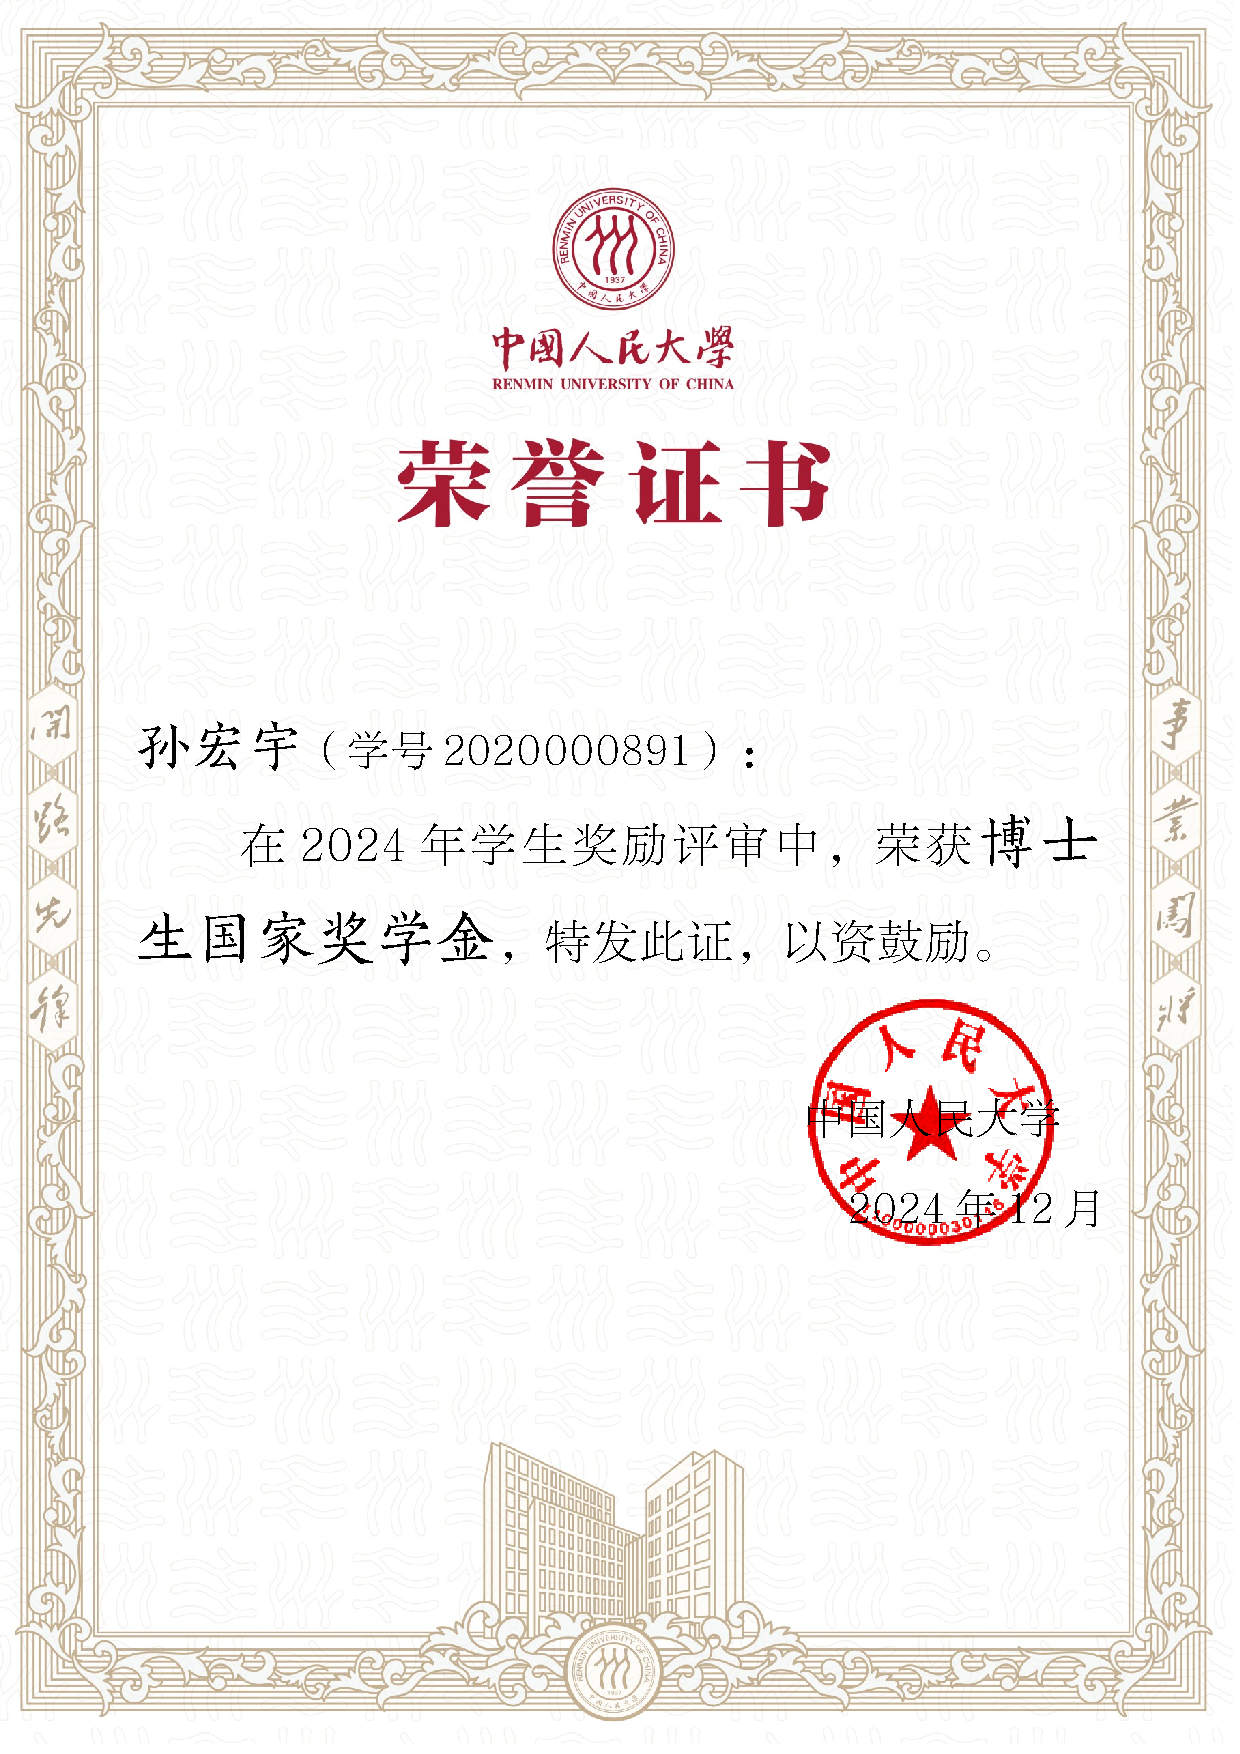
\includegraphics[width=\textwidth]{national_scholarhsip.pdf}
        %  \caption{Description of first image}
         \label{fig:image1}
     \end{subfigure}
     \hfill % Adds spacing between images
     % Second Image
     \begin{subfigure}[b]{0.32\textwidth}
         \centering
         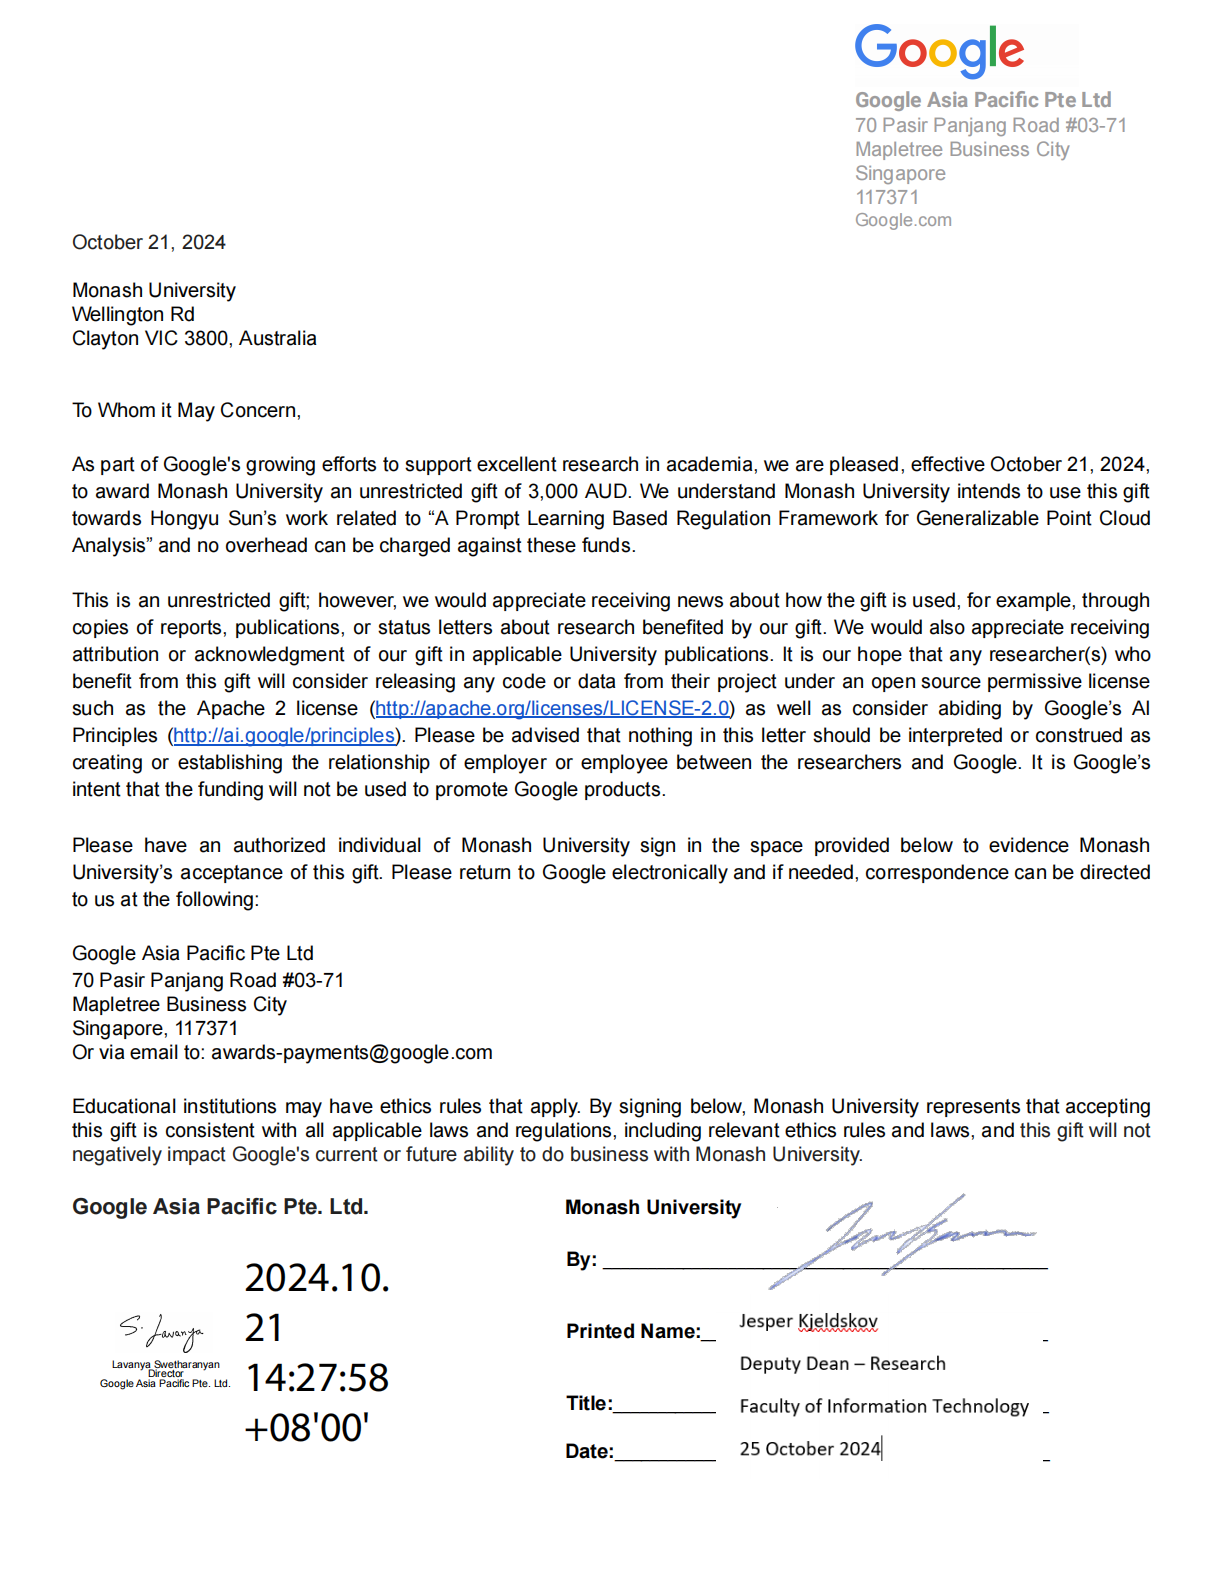
\includegraphics[width=\textwidth]{google_travel_grant.png}
        %  \caption{Description of second image}
         \label{fig:image2}
     \end{subfigure}
     \hfill % Adds spacing between images
     % Third Image
     \begin{subfigure}[b]{0.32\textwidth}
         \centering
         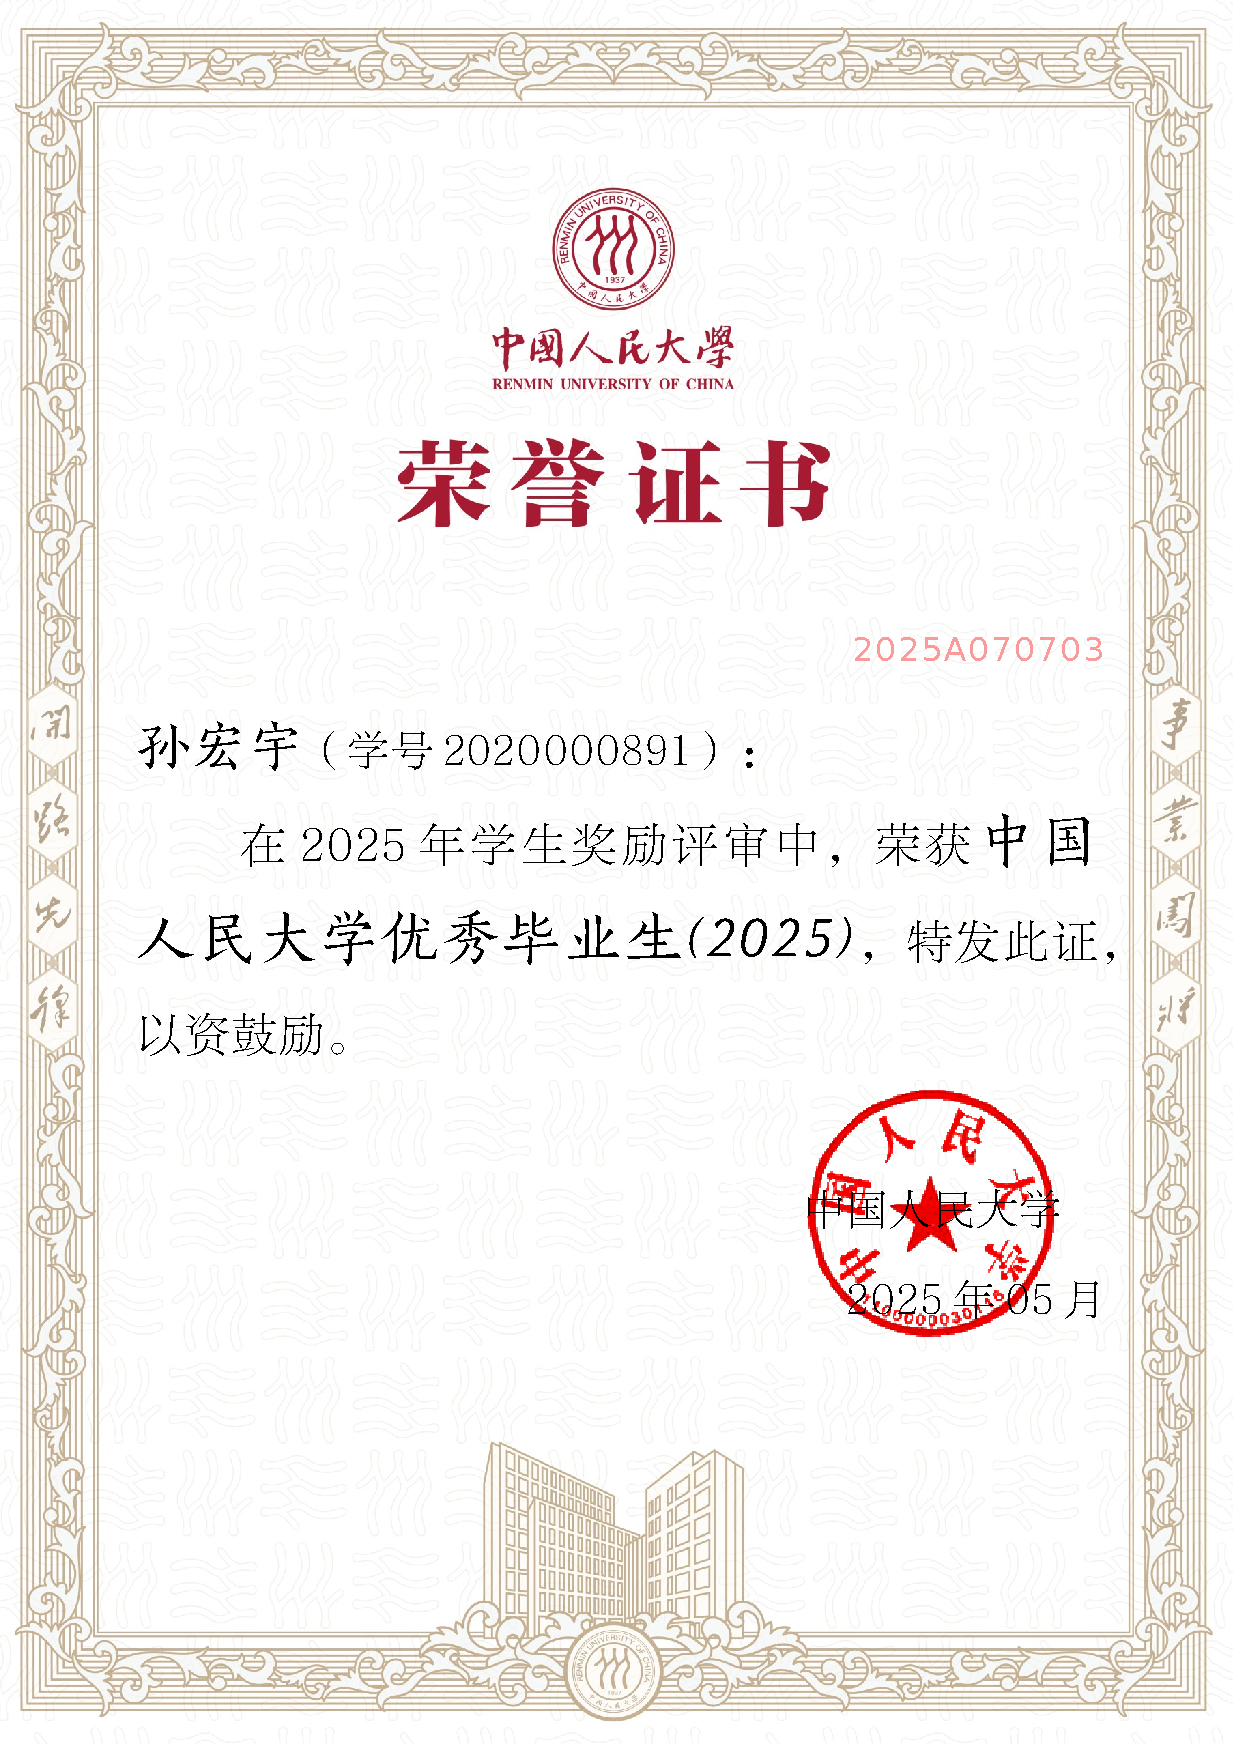
\includegraphics[width=\textwidth]{outstanding_doctoral_graduate.pdf}
        %  \caption{Description of third image}
         \label{fig:image3}
     \end{subfigure}
     
     \caption{博士期间科研工作获奖}
     \label{fig:three_graphs}
\end{figure}

\NsfcSection{2}{工作条件}{
（包括已具备的实验条件，尚缺少的实验条件和拟解决的途径，
包括利用国家实验室、
全国重点实验室和部门重点实验室等研究基地的计划与落实情况）；}

% 学校介绍
申请人的工作单位是内蒙古大学计算机学院。内蒙古大学作为国家“211工程”重点建设院校和国家“双一流”建设高校，具有较强的综合实力和较好的研究平台，是中国教育科研计算网（CERNET）和下一代互联网（CNGI-CERNET2）内蒙古地区主节点。内蒙古大学计算机学院现有计算机科学与技术一级学科博士点和博士后科研流动站，设有“蒙古文智能信息处理技术国家地方联合工程研究中心”和“生态大数据教育部工程中心”两个国家级和部委级科研平台。

% 时空智能中心
%   实验场地
申请人是内蒙古大学时空智能研究中心团队成员，该中心由\myEmph{计算机学院特聘院长、国家杰出青年基金获得者史振威教授}领衔。时空智能研究中心聚焦智慧生态、边防、交通、能源、应急等特色应用场景，深耕具有内蒙古地域特色的时空智能理论研究与技术转化。本项目围绕开放环境下3D点云处理方法的自适应问题开展研究，紧扣空间智能研究主题。
学校和学院为时空智能研究中心提供了800多平方米的办公场地，为项目执行和人员交流提供了良好环境。

%   实验设备
实验设备方面，申请人购买了有1个台式电脑、1个笔记本电脑、1台打印机。台式电脑配置为Intel Core i9-14900K CPU，192GB内存，2张NVIDIA RTX 5090显卡，12TB 硬盘存储空间；笔记本电脑配置为 Apple M4 Max 处理器，128GB内存，4TB固态硬盘。此外，时空智能研究中心有8台浪潮服务器，每台配置了4块 A100 GPU，申请人可以和其他成员共同使用。这些设备为本项目数据处理、模型设计、方法验证和迭代优化提供了稳定的存储和计算支撑。

% 软件和数据
软件工具方面，申请人具备搭建实验环境的实际经验，能够熟练使用 Linux、Docker、Git等操作系统和工具构建开发环境；申请人已掌握常用的编码工具（Python, C++, PyTorch）以及针对点云处理的专用软件（PyTorch3D\footnote{\url{https://github.com/facebookresearch/pytorch3d}}, Torch-Points3D\footnote{\url{https://github.com/torch-points3d/torch-points3d}}, Open3D\footnote{\url{https://github.com/isl-org/Open3D}}），实现点云处理模型的设计、训练、调试和可视化。

% 数据集
实验数据方面，申请人在读博士期间搜集了领域内大量公开的点云数据集，熟悉数据集的来源、格式、使用方法。点云物体识别方面，公开的数据集包括 ModelNet、ScanObjectNN、ShapeNet、OminObject3D、Objaverse 等；点云物体检测方面，有公开的室内场景数据集（ScanNet、SUN RGBD、S3DIS、ARKitScenes、MultiScan、3RScan）和室外场景数据集（KITTI、nuScenes、Waymo Open、ONCE、Argoverse 2）；点云场景语义分割方面，有室内场景数据集（S3DIS、ScanNet、Matterport3D、Structured3D、Replica）和室外场景数据集（SemanticKITTI、Semantic3D、SemanticPOSS、PandaSet、nuScenes (LidarSeg)、Waymo Open Dataset）。
这些经验和积累为本项目的执行和推进奠定了数据基础。

% 其他实验设备/耗材/劳务/差旅/专家咨询/论文版面和专利费
本项目中用到的其他小型计算设备、实验耗材的费用，以及研究人员劳务、参加学术会议、专家咨询、论文发表和申请专利涉及的费用，拟通过本项目申请的专项经费予以支持。

-----------------------

申请人受邀担任IEEE TPAMI, IJCV, IEEE CVPR, NeurIPS 等本领域多个顶级期刊和会议的审稿人。（***这句话想办法移到前面合适的地方***）

与这些国内外相关研究团队开展密切合作与交流的经验也将为项目的成功
进行起到重要的促进作用。

申请人所申报的项目将依托于内蒙古大学时空智能研究中心。
现有优越的实验条件可以充分满足项目研发需求。
项目团队将继续加强国际交流与合作，
以创新性的高水平学术成果为研究目标。

（1）在硬件条件方面，申请人所在的项目组有一台2卡RTX 5090 GPU服务器，内存256G，存储空间12T，满足了项目前期的数据处理和模型开发需求。
（2）在软件条件方面，申请人长期从事3D点云处理、模型鲁棒性和泛化性、测试时自适应技术方面的研究，以第一作者发表了多篇高水平论文，并将开发的算法和模型开源到GitHub社区（https://github.com/auniquesun/），受到同行广泛下载和使用，展示了出色的科研能力和扎实的工程技术能力；本项目参与者为深度学习和机器视觉的教学科研一线工作者，掌握了图像和点云处理相关的理论和方法，为本项目的执行奠定了坚实的理论和实践基础。
（3）在数据资源方面，目前学术界和工业界已有公开的点云和图像多模态数据集，如 SemanticKITTI, nuScenes, ShapeNet，Objaverse, OmniObject3D包含了城市道路场景、常见3D物体等数据，样本合计超过 100万，这些公开的数据为本项目前期算法模拟和测试提供了必要的数据基础。
（4）需要购买一台GPU服务器，用于满足本项目点云知识库构建、数据存储、测试时自适应技术开发、点云处理模型测试和部署等方面的需求。

\NsfcSection{3}{正在承担的与本项目相关的科研项目情况}{
（申请人正在承担的与本项目相关的科研项目情况，包括国家自然科学基金
的项目和国家其他科技计划项目，要注明项目的资助机构、项目类别、
批准号、项目名称、获资助金额、起止年月、与本项目的关系及负责
的内容等）；}

无

\NsfcSection{4}{完成国家自然科学基金项目情况}{
（对申请人负责的前一个已资助期满的科学基金项目（项目名称及批准号）完成情况、后续研究进
展及与本申请项目的关系加以详细说明。另附该项目的研究工作总结
摘要（限500字）和相关成果详细目录）。}

无

%%%%%%%%%%%%%%%%%%%%%%%%%%%%%%%%%%%%%%%%%%%%%%%%%
\ContentDes{（三） 其他需要说明的情况}



\NsfcSection{1}{}{申请人同年申请不同类型的国家自然科学基金项目情况（列明
同年申请的其他项目的项目类型、项目名称信息，并说明与本项目之
间的区别与联系；已收到自然科学基金委不予受理或不予资助决定的，
无需列出）。}

无

\NsfcSection{2}{}{具有高级专业技术职务（职称）的申请人是否
存在同年申请或者参与申请国家自然科学基金项目的单位不一致的情
况；如存在上述情况，列明所涉及人员的姓名，申请或参与申请的其
他项目的项目类型、项目名称、单位名称、上述人员在该项目中是申
请人还是参与者，并说明单位不一致原因。}

无

\NsfcSection{3}{}{具有高级专业技术职务（职称）的申请人是否
存在与正在承担的国家自然科学基金项目的单位不一致的情况；如存
在上述情况，列明所涉及人员的姓名，正在承担项目的批准号、项目
类型、项目名称、单位名称、起止年月，并说明单位不一致原因。}

无

\NsfcSection{4}{}{同年以不同专业技术职务（职称）申请或参与申请科学基金项
目的情况（应详细说明原因）。}

无

\NsfcSection{5}{}{其他。}

无


\end{document}
